% HBS fine fragmentation in SCIANTIX: roadmap and first results, with the RVE tests for MMM
% E. Cappellari -- meeting of 14 October 2026 (copy of mmm_runs.tex of 13 October, extended with context and NFIR results)
% Build: latexmk -pdf mmm_roadmap.tex      Figures from ../figures/ (python3 ../pore_distribution.py) and
%        ../../../regression/hbs_nfir/figures/j19damage/ (python3 regression/hbs_nfir/plot.py j19damage)

\documentclass[10pt,aspectratio=169]{beamer}
\usetheme[progressbar=frametitle,numbering=fraction,block=fill]{metropolis}
\usepackage{amsmath,amssymb,booktabs,graphicx,tikz}
\usetikzlibrary{arrows.meta,positioning}
\usepackage[T1]{fontenc}
\usepackage[utf8]{inputenc}
\graphicspath{{../figures/}{../../../regression/hbs_nfir/figures/j19damage/}}
\definecolor{paper}{RGB}{0,80,180}
\definecolor{own}{RGB}{190,50,40}
\definecolor{done}{RGB}{40,130,80}
\newcommand{\pp}[1]{{\color{paper}#1}}   % from a paper
\newcommand{\oo}[1]{{\color{own}#1}}     % our own choice
\newcommand{\dd}[1]{{\color{done}#1}}    % done
\setbeamertemplate{caption}{\raggedright\insertcaption\par}

\title{Fine fragmentation of the high-burnup structure in SCIANTIX}
\subtitle{Roadmap and first results}
\author{E.\ Cappellari}
\institute{POLIMI -- CEA}
\date{14 October 2026}

\begin{document}
\maketitle

% =====================================================================================================================
\section{Context}

% ---------------------------------------------------------------------------------------------------------------------
\begin{frame}{SCIANTIX \& HBS fragmentation modelling}
\begin{itemize}
\item HBS formation: restructured volume fraction $\alpha$
\item HBS porosity: pore density $N_p$, mean volume $\bar V$, Xe atoms per pore $\bar n$ and their variance $\mathrm{Var}(n)$
\item \oo{HBS fragmentation}: which pores break, how much gas they release, fragment size
\end{itemize}

\textbf{Rupture per pore class, progressive}
\begin{itemize}
\item 81 pore classes rebuilt at every step from the state of the porosity model: $(\bar V,\bar n,\mathrm{Var}(n))$
\item a rupture criterion on every class; the broken classes vent their content
\item outputs: $D$ = fraction of broken pores (fragment size), $G$ = fraction of the pore gas released,
      $d$ = mean fragment size
\item no parameter fitted on the test shown below
\end{itemize}
\end{frame}

% ---------------------------------------------------------------------------------------------------------------------
\begin{frame}{Rupture criterion: Jernkvist 2019 and OperaHPC D5.2}
\vspace{-4pt}
\[
\oo{\hat s\,\bigl(p-\tfrac{2\gamma}{R}-P_h\bigr)\ \ge\ \sigma_R+P_h}
\quad\Longleftrightarrow\quad
p\ge P_{cr}=P_h+\frac{2\gamma}{R}+\frac{\sigma_R+P_h}{\hat s}
\]
\vspace{6pt}

\begin{columns}[T]
\column{0.49\linewidth}
\pp{Jernkvist 2019} (Olander)
\vspace{4pt}
\[
\pp{P_{cr}=\frac{2\gamma}{R}+\frac{\sigma^{cr}_{hbs}(1-\xi)+P_h}{\xi}},
\]
\vspace{-8pt}
\[
\sigma^{cr}_{hbs}=21\ \text{MPa} \quad \hat s=\frac{\xi}{1-\xi}
\]
\column{0.49\linewidth}
\pp{OperaHPC D5.2}
\vspace{4pt}
\[
\pp{\sigma_I^{max}\big|_i\ge\sigma_R=275\ \text{MPa}},
\]
\vspace{-8pt}
\[
\hat s_i=\frac{\sigma_I^{max}|_i(1,p_{hyd})+p_{hyd}}{1-p_{hyd}}
\]
\end{columns}
\vspace{4pt}
\small
$\hat s$ is the stress concentration factor at the pore that will enter in SCIANTIX following micromechanics calculation. Everything else in the criterion comes from the SCIANTIX state.
\end{frame}

% ---------------------------------------------------------------------------------------------------------------------
\begin{frame}{Scope and chain of tools}
Goal: replace the mean-field stress factor $\xi/(1-\xi)$ of Jernkvist by tables computed with MMM on RVEs that reproduce
the pore classes that SCIANTIX will see.
\vspace{6pt}

\centering
\resizebox{\linewidth}{!}{%
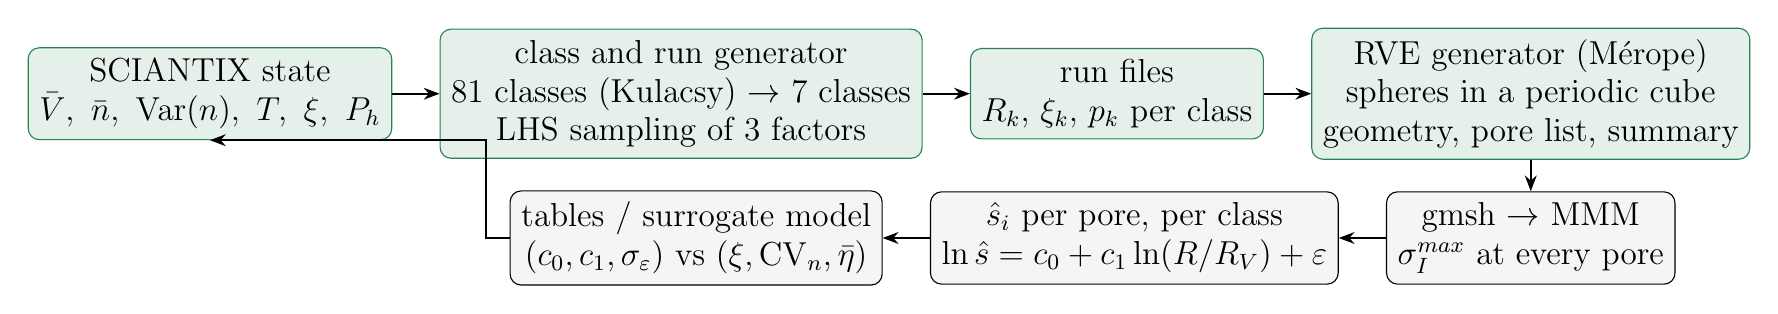
\begin{tikzpicture}[node distance=4mm and 6mm, every node/.style={font=\large},
  box/.style={draw, rounded corners, align=center, minimum height=9mm, inner sep=4pt, fill=black!4},
  dbox/.style={box, fill=done!12, draw=done},
  arr/.style={-{Stealth[length=2mm]}, thick}]
\node[dbox] (sx) {SCIANTIX state\\ $\bar V,\ \bar n,\ \mathrm{Var}(n),\ T,\ \xi,\ P_h$};
\node[dbox, right=of sx] (pd) {class and run generator\\ 81 classes (Kulacsy) $\to$ 7 classes\\ LHS sampling of 3 factors};
\node[dbox, right=of pd] (rf) {run files\\ $R_k$, $\xi_k$, $p_k$ per class};
\node[dbox, right=of rf] (me) {RVE generator (M\'erope)\\ spheres in a periodic cube\\ geometry, pore list, summary};
\node[box, below=of me] (gm) {gmsh $\to$ MMM \\ $\sigma_I^{max}$ at every pore};
\node[box, left=of gm] (fit) {$\hat s_i$ per pore, per class\\ $\ln\hat s=c_0+c_1\ln(R/R_V)+\varepsilon$};
\node[box, left=of fit] (tab) {tables / surrogate model \\ $(c_0,c_1,\sigma_\varepsilon)$ vs $(\xi,\mathrm{CV}_n,\bar\eta)$};
\draw[arr] (sx) -- (pd); \draw[arr] (pd) -- (rf); \draw[arr] (rf) -- (me); \draw[arr] (me) -- (gm);
\draw[arr] (gm) -- (fit); \draw[arr] (fit) -- (tab); \draw[arr] (tab.west) -| ++(-3mm,0) |- (sx.south);
\end{tikzpicture}}
\vspace{4pt}

\small \dd{green: done}; grey: next.
\end{frame}

% ---------------------------------------------------------------------------------------------------------------------
\begin{frame}{Pore classes from SCIANTIX - Pore population generator I}
\small
Porosity model from SCIANTIX: $\bar V$ ($R_V$), $\bar n$ = Xe-atoms/pore, $\mathrm{Var}(n)$, $N_p$, $\xi=N_p\bar V$.
\vspace{2pt}
{\footnotesize
\begin{align*}
\pp{\text{log-normal R (K15)}}&:\quad 81\text{ nodes } x_i\in[-4,4],\quad w_i\propto e^{-x_i^2/2},\quad
R_i=R_V\,e^{s x_i}\Big/\bigl(\textstyle\sum_j w_j e^{3 s x_j}\bigr)^{1/3}\ \ (\textstyle\sum_i w_iV_i=\bar V)\\
\oo{\text{Xe/pore distribution}}&:\quad n_i=\bar n\,R_i^{a}\Big/\textstyle\sum_j w_jR_j^{a},\quad a=2\ (\text{gas density}\propto1/R),\qquad
s\ \text{from}\ \textstyle\sum_i w_i(n_i-\bar n)^2=\mathrm{Var}(n)\\
\text{pressure distribution}&:\quad p_i=\frac{n_ik_BT}{V_i}\,Z(\eta_i),\qquad \eta_i=\min\!\Bigl(\frac{n_iv_{Xe}(T)}{V_i},0.65\Bigr)\quad\text{hard spheres}
\end{align*}}
\vspace{-8pt}
\centering\includegraphics[width=\linewidth]{classes_distributions.png}

\scriptsize NFIR, end of base irradiation: $s=0.33$ (measured about 0.3, K15 0.356), radii 0.08--1.1 $\mu$m, $p_i$ from 2.7 GPa to 30 MPa.
\end{frame}

% ---------------------------------------------------------------------------------------------------------------------
\begin{frame}{Pore population generator II}
\small
\begin{align*}
\sum_iw_iV_i&=\bar V && \text{exact by construction}\\
\sum_iw_in_i&=\bar n && \text{exact by construction}\\
\mathrm{CV}_n^2(s,a)&=\frac{\sum_iw_ie^{2asx_i}}{\bigl(\sum_iw_ie^{asx_i}\bigr)^2}-1=\frac{\mathrm{Var}(n)}{\bar n^2} && \text{root in }s
\end{align*}
Mean pressure (pressure of the volume-weighted density): $p_{EoS}(\bar n,\bar V,T)$ is conserved. 

\centering\includegraphics[width=0.9\linewidth]{classes_moment_errors.png}
\end{frame}

% ---------------------------------------------------------------------------------------------------------------------
\begin{frame}{Pore population generator III: Xe atoms/pore}
\includegraphics[width=0.4\textwidth]{classes_closure_exponent.png}
\includegraphics[width=0.59\textwidth]{classes_heatup.png}
\vspace{2pt}
\centering
The moments hold for every $a$; what changes is the width $s$, the pressure spread and which classes break: small pores first for $a<3$, while for $a=3$ uniform pressure.
\end{frame}

% ---------------------------------------------------------------------------------------------------------------------
\begin{frame}{Reduction of the parameter space and design of the runs}
 
MMM is scale-free in length and linear in the load: $R_V$ and $\bar p$ only set the scale. With $p^*=p\,v_{Xe}/k_BT$,
\[
p_i^*=\eta_iZ(\eta_i),\qquad \bar\eta=\frac{\bar n\,v_{Xe}(T)}{\bar V},\qquad \mathrm{CV}_n=\frac{\sqrt{\mathrm{Var}(n)}}{\bar n}
\]
so in $x_i=R_i/R_V$ the profile $p_i/\bar p$ and the weights $w_i$ depend on $(\bar\eta,\mathrm{CV}_n,a)$ only.

\begin{tabular}{@{}llc@{}}
\toprule
factor & sets & range \\
\midrule
$\xi$ & porosity, pore distances & 0.02--0.18 \\
$s$ (from $\mathrm{CV}_n$) & $R_k/R_V$ and $\xi_k/\xi$ & 0.05--0.42 \\
$\bar\eta$ & with $s$, the profile $p_k/\bar p$ & 0.045--0.23 \\
\bottomrule
\end{tabular}
 
Latin Hypercube Sampling: 7 pore classes per run (groups the 81 SCIANTIX nodes); 
Scale: $R_V=0.73\ \mu$m of the disc and the temperature of the anneal. Ranges from SCIANTIX on the NFIR history and from the measured disc; $\xi$ below 0.02 leaves less than two pores in the smallest class.

\end{frame}

\begin{frame}
      
\centering\includegraphics[width=\linewidth]{mmm_design.png}
\end{frame}

% ---------------------------------------------------------------------------------------------------------------------
\begin{frame}{M\'erope: geometry of a run}

For every run file:
\begin{enumerate}
\item read the classes, sort by decreasing radius
\item expected pores per class $=\xi_k/V_k\cdot L^3$
\item throw the spheres by RSA in a periodic cube, with a repulsion distance between surfaces
\item each sphere takes the class of the nearest radius, hence its pressure; one phase id per sphere, not meshed
\item write, per run and seed: the pore list (id, $x,y,z$, $R$, $p$), the .geo for gmsh, a summary
\end{enumerate}
Fixed:\\[4pt]
\begin{tabular}{@{}lll@{}}
\toprule
cube & 30 $\mu$m & $41\,R_V$ of the disc\\
repulsion & 0.3 $\mu$m & one HBS grain, as OperaHPC \\
mesh & 0.15 $\mu$m & as OperaHPC \\
seed & 1 per run & \\
\bottomrule
\end{tabular}
\end{frame}

% ---------------------------------------------------------------------------------------------------------------------
\begin{frame}{Tests on the RVE: size and mesh}
\footnotesize
Quantity under test: $Z_k$, the mean of $\hat s$ over the pores of class $k$ in a cube.
The proposed tests follow \pp{Kanit et al.\ 2003} (Int.\ J.\ Solids Struct.\ 40, 3647) and the work done in OperaHPC. %Worst case \oo{[R]}: R13, the run with the fewest and largest pores (Kanit Eq.\ 72): $\xi=0.04$, radii 0.23--1.68 $\mu$m. Load: one unit pressure in all the pores, as OperaHPC \oo{[R]}. 11 cubes, with their own geometry: independent of the 20 runs.
\vspace{4pt}

\begin{columns}[T]
\column{0.5\linewidth}
\textbf{Test 1: size of the cube}
\begin{itemize}
\item \textbf{base}: 10 cubes of 30 $\mu$m (different seeds), mesh 0.15 $\mu$m
\item scatter $D$ of $Z_k$ between the 10 cubes: the
      30 $\mu$m cube is an RVE for class $k$ if $2D/\bar Z\le $ Error \% 
%\item if not: $n=(2D/\bar Z\varepsilon)^2$ cubes (Eq.\ 70), side of the RVE from $D^2(V)=S^2A/V$ (Eq.\ 62)
% \item \textbf{exploration}, only if needed: 10 cubes of 20 $\mu$m (second variance: $A$, and $\alpha$ to $\pm0.55$;
%       rarest class still 1.2 pores per cube) and 2 of 40 $\mu$m (bias of the 30 $\mu$m cube)
\end{itemize}
\column{0.48\linewidth}
\textbf{Test 2: size of the mesh}
\begin{itemize}
\item a base cube re-meshed at 0.30 $\mu$m, the same pores; compared with its 0.15 $\mu$m twin
\item $\hat s$ pore by pore and the mean of every class on the two meshes
\item The corser mesh could be tested against the standard one, and also it can be refined within mmm to save computational cost. 
\end{itemize}
\end{columns}
\end{frame}

% ---------------------------------------------------------------------------------------------------------------------
% ---------------------------------------------------------------------------------------------------------------------
\begin{frame}{NFIR test}
\textbf{The test} \pp{(Noirot 2014; OperaHPC D5.2)}
\begin{itemize}
\item UO$_2$ disc irradiated in Halden to 103 GWd/t at 560--700 $^\circ$C, HBS over the whole disc, porosity 11 \%,
      88 \% of the remaining Xe in HBS pores
\item measured: pore size distribution before and after, gas density in the pores, temperature history
\item anneal: ramp to 300 $^\circ$C, hold, ramp to 1200 $^\circ$C at 0.2 $^\circ$C/s, hold 15 min; Kr-85 release online
\item release of about 30 \% of the gas produced, in two steps above 880 $^\circ$C, nothing during the hold; the disc
      breaks into pieces below 100 $\mu$m
\end{itemize}
State at the end of the base irradiation from SCIANTIX: $\xi=0.105$, $R_V=0.35\ \mu$m, $\bar n=7.2\times10^{8}$ Xe/pore, $\mathrm{CV}_n=0.75$
(measured disc: $R_V=0.73\ \mu$m, 1.7 times the gas density)
\end{frame}

% ---------------------------------------------------------------------------------------------------------------------
\begin{frame}{How SCIANTIX performs on NFIR: release}
No parameter fit
\includegraphics[width=\linewidth]{classes_fgr_nfir_j19damage.png}
\end{frame}

\begin{frame}{How SCIANTIX performs on NFIR: release}
No parameter fit
\includegraphics[width=0.8\linewidth]{classes_rupture_nfir_j19damage.png}
\end{frame}

% =====================================================================================================================
\section{Roadmap}

% ---------------------------------------------------------------------------------------------------------------------
\begin{frame}{Roadmap}
\footnotesize
\begin{columns}[T]
\column{0.49\linewidth}
\dd{\textbf{Done}}
\begin{itemize}
\item Draft model implemented in SCIANTIX 
\item NFIR anneal: release 39 \% of the measured, wrong shape; the levers identified
\item pore classes determined from the moments, LHS spans for all the factors
\item M\'erope geometry of the runs; proposed two RVE tests
\end{itemize}
\vspace{4pt}
\column{0.49\linewidth}
\textbf{Next, in order}
\begin{enumerate}
\item test on RVE size and mesh on the 11 cubes: cost of a cube, format of the output, RVE and mesh verdicts;
\item fill the LHS script with the RVE and mesh verdicts, run Merope for the cases: $\hat s_i$ per pore class
\item tables / surrogate $(c_0,c_1,\sigma_\varepsilon)$ against $(\xi,\mathrm{CV}_n,\bar\eta)$; 
\item validation runs outside the LHS
\item tables / surrogate into sciantix;
\end{enumerate}
\end{columns}
\end{frame}

\end{document}
